\documentclass{lni}


%\IfFileExists{latin1.sty}{\usepackage{latin1}}{\usepackage{isolatin1}}
\usepackage[latin1]{inputenc}
% Verwenden von T1 Fonts
\usepackage[T1]{fontenc}
\usepackage[ngerman]{babel}
\usepackage{graphicx}
\usepackage{amsmath}
\usepackage{amssymb}
\usepackage{listings}
%\usepackage{hyperref}
\usepackage{fancyvrb}
\usepackage{color}
\usepackage{algorithmic}
\usepackage{algorithm}
\usepackage{float}

\floatstyle{ruled}
\newfloat{program}{H}{lop}
\floatname{program}{Listing}

\makeatletter
\def\PY@reset{\let\PY@it=\relax \let\PY@bf=\relax%
    \let\PY@ul=\relax \let\PY@tc=\relax%
    \let\PY@bc=\relax \let\PY@ff=\relax}
\def\PY@tok#1{\csname PY@tok@#1\endcsname}
\def\PY@toks#1+{\ifx\relax#1\empty\else%
    \PY@tok{#1}\expandafter\PY@toks\fi}
\def\PY@do#1{\PY@bc{\PY@tc{\PY@ul{%
    \PY@it{\PY@bf{\PY@ff{#1}}}}}}}
\def\PY#1#2{\PY@reset\PY@toks#1+\relax+\PY@do{#2}}

\def\PY@tok@gd{\def\PY@tc##1{\textcolor[rgb]{0.63,0.00,0.00}{##1}}}
\def\PY@tok@gu{\let\PY@bf=\textbf\def\PY@tc##1{\textcolor[rgb]{0.50,0.00,0.50}{##1}}}
\def\PY@tok@gt{\def\PY@tc##1{\textcolor[rgb]{0.00,0.25,0.82}{##1}}}
\def\PY@tok@gs{\let\PY@bf=\textbf}
\def\PY@tok@gr{\def\PY@tc##1{\textcolor[rgb]{1.00,0.00,0.00}{##1}}}
\def\PY@tok@cm{\let\PY@it=\textit\def\PY@tc##1{\textcolor[rgb]{0.25,0.50,0.50}{##1}}}
\def\PY@tok@vg{\def\PY@tc##1{\textcolor[rgb]{0.10,0.09,0.49}{##1}}}
\def\PY@tok@m{\def\PY@tc##1{\textcolor[rgb]{0.40,0.40,0.40}{##1}}}
\def\PY@tok@mh{\def\PY@tc##1{\textcolor[rgb]{0.40,0.40,0.40}{##1}}}
\def\PY@tok@go{\def\PY@tc##1{\textcolor[rgb]{0.50,0.50,0.50}{##1}}}
\def\PY@tok@ge{\let\PY@it=\textit}
\def\PY@tok@vc{\def\PY@tc##1{\textcolor[rgb]{0.10,0.09,0.49}{##1}}}
\def\PY@tok@il{\def\PY@tc##1{\textcolor[rgb]{0.40,0.40,0.40}{##1}}}
\def\PY@tok@cs{\let\PY@it=\textit\def\PY@tc##1{\textcolor[rgb]{0.25,0.50,0.50}{##1}}}
\def\PY@tok@cp{\def\PY@tc##1{\textcolor[rgb]{0.74,0.48,0.00}{##1}}}
\def\PY@tok@gi{\def\PY@tc##1{\textcolor[rgb]{0.00,0.63,0.00}{##1}}}
\def\PY@tok@gh{\let\PY@bf=\textbf\def\PY@tc##1{\textcolor[rgb]{0.00,0.00,0.50}{##1}}}
\def\PY@tok@ni{\let\PY@bf=\textbf\def\PY@tc##1{\textcolor[rgb]{0.60,0.60,0.60}{##1}}}
\def\PY@tok@nl{\def\PY@tc##1{\textcolor[rgb]{0.63,0.63,0.00}{##1}}}
\def\PY@tok@nn{\let\PY@bf=\textbf\def\PY@tc##1{\textcolor[rgb]{0.00,0.00,1.00}{##1}}}
\def\PY@tok@no{\def\PY@tc##1{\textcolor[rgb]{0.53,0.00,0.00}{##1}}}
\def\PY@tok@na{\def\PY@tc##1{\textcolor[rgb]{0.49,0.56,0.16}{##1}}}
\def\PY@tok@nb{\def\PY@tc##1{\textcolor[rgb]{0.00,0.50,0.00}{##1}}}
\def\PY@tok@nc{\let\PY@bf=\textbf\def\PY@tc##1{\textcolor[rgb]{0.00,0.00,1.00}{##1}}}
\def\PY@tok@nd{\def\PY@tc##1{\textcolor[rgb]{0.67,0.13,1.00}{##1}}}
\def\PY@tok@ne{\let\PY@bf=\textbf\def\PY@tc##1{\textcolor[rgb]{0.82,0.25,0.23}{##1}}}
\def\PY@tok@nf{\def\PY@tc##1{\textcolor[rgb]{0.00,0.00,1.00}{##1}}}
\def\PY@tok@si{\let\PY@bf=\textbf\def\PY@tc##1{\textcolor[rgb]{0.73,0.40,0.53}{##1}}}
\def\PY@tok@s2{\def\PY@tc##1{\textcolor[rgb]{0.73,0.13,0.13}{##1}}}
\def\PY@tok@vi{\def\PY@tc##1{\textcolor[rgb]{0.10,0.09,0.49}{##1}}}
\def\PY@tok@nt{\let\PY@bf=\textbf\def\PY@tc##1{\textcolor[rgb]{0.00,0.50,0.00}{##1}}}
\def\PY@tok@nv{\def\PY@tc##1{\textcolor[rgb]{0.10,0.09,0.49}{##1}}}
\def\PY@tok@s1{\def\PY@tc##1{\textcolor[rgb]{0.73,0.13,0.13}{##1}}}
\def\PY@tok@sh{\def\PY@tc##1{\textcolor[rgb]{0.73,0.13,0.13}{##1}}}
\def\PY@tok@sc{\def\PY@tc##1{\textcolor[rgb]{0.73,0.13,0.13}{##1}}}
\def\PY@tok@sx{\def\PY@tc##1{\textcolor[rgb]{0.00,0.50,0.00}{##1}}}
\def\PY@tok@bp{\def\PY@tc##1{\textcolor[rgb]{0.00,0.50,0.00}{##1}}}
\def\PY@tok@c1{\let\PY@it=\textit\def\PY@tc##1{\textcolor[rgb]{0.25,0.50,0.50}{##1}}}
\def\PY@tok@kc{\let\PY@bf=\textbf\def\PY@tc##1{\textcolor[rgb]{0.00,0.50,0.00}{##1}}}
\def\PY@tok@c{\let\PY@it=\textit\def\PY@tc##1{\textcolor[rgb]{0.25,0.50,0.50}{##1}}}
\def\PY@tok@mf{\def\PY@tc##1{\textcolor[rgb]{0.40,0.40,0.40}{##1}}}
\def\PY@tok@err{\def\PY@bc##1{\fcolorbox[rgb]{1.00,0.00,0.00}{1,1,1}{##1}}}
\def\PY@tok@kd{\let\PY@bf=\textbf\def\PY@tc##1{\textcolor[rgb]{0.00,0.50,0.00}{##1}}}
\def\PY@tok@ss{\def\PY@tc##1{\textcolor[rgb]{0.10,0.09,0.49}{##1}}}
\def\PY@tok@sr{\def\PY@tc##1{\textcolor[rgb]{0.73,0.40,0.53}{##1}}}
\def\PY@tok@mo{\def\PY@tc##1{\textcolor[rgb]{0.40,0.40,0.40}{##1}}}
\def\PY@tok@kn{\let\PY@bf=\textbf\def\PY@tc##1{\textcolor[rgb]{0.00,0.50,0.00}{##1}}}
\def\PY@tok@mi{\def\PY@tc##1{\textcolor[rgb]{0.40,0.40,0.40}{##1}}}
\def\PY@tok@gp{\let\PY@bf=\textbf\def\PY@tc##1{\textcolor[rgb]{0.00,0.00,0.50}{##1}}}
\def\PY@tok@o{\def\PY@tc##1{\textcolor[rgb]{0.40,0.40,0.40}{##1}}}
\def\PY@tok@kr{\let\PY@bf=\textbf\def\PY@tc##1{\textcolor[rgb]{0.00,0.50,0.00}{##1}}}
\def\PY@tok@s{\def\PY@tc##1{\textcolor[rgb]{0.73,0.13,0.13}{##1}}}
\def\PY@tok@kp{\def\PY@tc##1{\textcolor[rgb]{0.00,0.50,0.00}{##1}}}
\def\PY@tok@w{\def\PY@tc##1{\textcolor[rgb]{0.73,0.73,0.73}{##1}}}
\def\PY@tok@kt{\def\PY@tc##1{\textcolor[rgb]{0.69,0.00,0.25}{##1}}}
\def\PY@tok@ow{\let\PY@bf=\textbf\def\PY@tc##1{\textcolor[rgb]{0.67,0.13,1.00}{##1}}}
\def\PY@tok@sb{\def\PY@tc##1{\textcolor[rgb]{0.73,0.13,0.13}{##1}}}
\def\PY@tok@k{\let\PY@bf=\textbf\def\PY@tc##1{\textcolor[rgb]{0.00,0.50,0.00}{##1}}}
\def\PY@tok@se{\let\PY@bf=\textbf\def\PY@tc##1{\textcolor[rgb]{0.73,0.40,0.13}{##1}}}
\def\PY@tok@sd{\let\PY@it=\textit\def\PY@tc##1{\textcolor[rgb]{0.73,0.13,0.13}{##1}}}

\def\PYZbs{\char`\\}
\def\PYZus{\char`\_}
\def\PYZob{\char`\{}
\def\PYZcb{\char`\}}
\def\PYZca{\char`\^}
\def\PYZsh{\char`\#}
\def\PYZpc{\char`\%}
\def\PYZdl{\char`\$}
\def\PYZti{\char`\~}
% for compatibility with earlier versions
\def\PYZat{@}
\def\PYZlb{[}
\def\PYZrb{]}
\makeatother

\usepackage{lastpage}
\thispagestyle{plain}
\pagenumbering{arabic}


\author{
	peterrr, Lusy \\
	\\
	%Abteilung \\
	Freie Universit�t Berlin \\
	%Anschrift \\
	%Postleitzahl Ort \\
	emaiaddresse@autor1 \\
	emaiaddresse@autor2
}
\title{Auffinden von Assoziationsregeln zwischen Themen in wissenschaftlichen Publikationen}

\newtheorem{mdef}{Definition}
\begin{document}
\maketitle

\begin{abstract}
Mit Hilfe der Assoziationsanalyse sollen Beziehungen zwischen Themen von wissenschaftlichen Publikationen gefunden werden. Hierf�r wird auf den aprior-Algorithmus zur�ckgegriffen. Der Analyse zugrundeliegende Datensatz waren alle Publikationen von arxiv.org mit dem Stand Oktober 2011. Die gefundenen Beziehungen k�nnen, unter anderem, f�r Erstellung von Recommendersystemen oder Mappings zwischen verschiedenen wissenschaftlichen Klassifikationen genutzt werden.
\end{abstract}

\tableofcontents
\newpage
%-------------------------------------------------------
%----Hauptteil------------------------------------------
%-------------------------------------------------------

\section{Einleitung}
\subsection{Motivation}
In Anlehnung an die Warenkorbanalyse sollen die vergebenen Themen f�r wissenschaftliche Publikationen analysiert werden,
um so h�ufig miteinander vergebene Themen und Br�ckenthemen zwischen Fachgebieten zu ermitteln.
Zusammen mit der Ermittlung von Koautorengraphen und der Zitationsanalyse ist die Analyse von Themen eine der Hauptmethoden der Bibliometrie.
Eine Untersuchung der Themenvergabe von wissenschaftlichen Publikationen kann interessante Erkenntnisse liefern, um die zeitliche Entwicklung bestimmten Themengebieten zu verfolgen oder verwandte Publikationen zu ermitteln.
\subsection{Problemstellung}
In dieser Arbeit werden die Themen zu wissenschaftlichen Publikationen anhand der ver�ffentlichten Publikationen auf arXiv.org zum 01.10.2011 beispielhaft untersucht.
Das Verfahren, um Beziehungen zwischen Themen zu finden, ist die Assoziationsanalyse.
Durch Assoziationsregeln k�nnen Themen, die oft zusammen auftreten, schnell aufgedeckt werden, bzw. vorhandenen Korrelationen und Abh�ngigkeiten zwischen ihnen ermittelt werden.
Durch eine geeignete Sortierung nach den verschiedenen Kenngr��en f�r Assoziationsregeln - Support, Konfidenz und Lift, k�nnen wir ferner die wichtigsten oder am h�ufigsten im Datensatz vorkommenden Regeln bestimmen.
Das durch diese Analyse gewonnene Wissen kann sp�ter f�r den Entwurf eines Paperrecommendersysstems oder das Erstellen eines geeigneten und zuverl�ssigen Mappings zwischen verschiedenen wissenschaftlichen Klassifikationen verwendet werden.
\\
\\
Unser Analyseansatz basiert auf \cite{Agrawal:1993:MAR:170035.170072} und die Auswertungen wurden mit Hilfe der Programmiersprache $R$ durchgef�hrt.
F�r das Parsen der XML-Daten benutzen wir einen in $Python$ geschriebenen Parser.

\subsection{Aufbau dieses Papers}
Im Weiteren wird dieses Dokument folgenderma�en aufgebaut:\newline
Kapitel 2 stellt die theoretischen Grundlagen der Assoziationsanalyse vor und erkl�rt den apriori-Algorithmus, den wir f�r die Extraktion der Assoziationsregeln in unserer Arbeit benutzen.
Im Kapitel 3 beschreiben wir die Merkmale und Besonderheiten des arxiv.org Datensatzes, sowie wie wir diesen weiter verarbeitet haben.
In Kapitel 4 geben wir eine detaillierte Auswertung der gefundenen Ergebnisse.
Kapitel 5 schl�gt weitere Aspekte vor, die erforscht werden k�nnen, und betrachtet zugleich m�gliche Anwendungen der Forschungsergebnisse.
In Kapitel 6 wird nochmal eine abschlie�ende Zusammenfassung der Arbeit aufgef�hrt.

%-present the subject, it could be with an example
%-define the important words
%-present the hypothesis + arguments etc.
%-describe how the body is organized

%Quite literally, the Introduction must answer the questions, "What was I studying? Why was it an important question? What did we know about it before I did this study? How will this study advance our knowledge?"


\section{Assozationsanalyse}\cite{Agrawal:1993:MAR:170035.170072}% TODO test um unser Startpaper zu zitieren
Die Assoziationanalyse beschreibt die Suche nach Assoziationsregeln innnerhalb einer Menge von Transaktionen. Transaktionen sind endliche Teilmengen aus einer sogenannten Itemmenge. Items sind Objekte, die in Transaktionen auftreten können. Ein Datensatz zur Assoziationsanalyse besteht also aus einer Menge von Transaktionen.
\subsection{Assozationsregeln}
Assoziationsregeln sind Implikationen der Form $A \rightarrow B$ und beschreiben den Sachverhalt, dass wenn $A$ auftritt auch $B$ auftritt.
\subsection{Kenngrößen von Assoziationsregeln}
\subsubsection{Support}
Der Support bezeichnet die relative Häufigkeit des Auftretens der Itemmenge $X$ in einem Datensatz.
\begin{mdef}[Support]
\[
\mathrm{support}(X) = \frac{\text{Anzahl der vorkommen von X im Datensatz}}{\text{Anzahl aller Transaktionen}}
\]
\end{mdef}
\subsubsection{Konfidenz}
Die Konfidenz ist die relative Häufigkeit der Transaktionen in denen X zusammen mit Y vorkommt. Oder anders formuliert, beschreibt diese, wie oft Y vorkommt, gegeben dass X vorkommt.
\begin{mdef}[Konfidenz]
\[
\mathrm{conf}(X\rightarrow Y) = \frac{\mathrm{support}(X \cup Y)}{\mathrm{support}(X)}
\]
\end{mdef}
\subsubsection{Lift}
Der Lift wird für die Stärke einer Regel bzw. deren Bedeutung herrangezogen.
\begin{mdef}[Lift]
\[
\mathrm{lift}(X\rightarrow Y) = \frac{ \mathrm{support}(X \cup Y)}{ \mathrm{support}(Y) \cdot \mathrm{support}(X) }
\]
\end{mdef}
\subsection{apriori-Algorithmus}
Der apriori-Algorithmus wurde 1994 von \cite{Agrawal:1994:FAM:645920.672836}  veröffentlicht, der sich fundamental zu denbis dato existierenden Algorithmen zum Finden von Assoziationsregeln unterscheidet. \\
$I = \{i_1, i_2, \ldots i_m\}$ ist eine endliche Menge von Items, die in einer Transaktion vorkommen können.
$D = \{t_1, t_2, \ldots , t_n\}$ ist eine Menge von Transaktionen, wobei jede Transaktion $T \subset I$ ein Teilmenge der Menge von Items ist. Weiterhin wird ein minimaler Support $\mathrm{minsupp}$ und eine minimale Konfidenz $\mathrm{minconf}$ definiert, die als Kriterium für die Assoziationsregeln verwendet wird. Der Algorithmus wird in zwei Probleme aufgeteilt.
\begin{description}
	\item[Problem 1] Finden aller Teilmengen von Items in die Transaktionen, die mindestens einen Support von $\mathrm{minsupp}$ haben.
	\item[Problem 2] Aus den gefundenen Teilmengen in Problem 1 werden Assoziationsregeln erzeugt. Nur Regeln, die mindestens eine Konfidenz von $\mathrm{minconf}$ haben, werden berücksichtigt.
\end{description}
\subsubsection{Finden von häufigen Mengen}
Sei $L_k$ die Menge aller Mengen mit k Items, die mindestens einen Support von $\mathrm{minsupp}$ haben, und $C_k$ die Menge möglicher Kandidaten für $L_k$. Im ersten Schritt wird die Häufigkeit aller Items in den Transaktionen aus $D$ berechnet und die Items, die mindestens $\mathrm{minsupp}$ haben, bilden $L_1$. In der k-ten Iteration werden neue Kandidaten für $L-k$ erzeugt und wenn diese wieder $\mathrm{minsupp}$ übersteigen, werden sie in $L_k$ aufgenommen. Der Algorithmus terminiert, wenn keine der erzeugten Kandidatenmengen in $L_k$ aufgenommen wurde, also $L_k = \emptyset$.
\begin{algorithm}
	\caption{apriori Algorithmus}
	\label{apriori}
\begin{algorithmic}
	\STATE $L_1\gets \{\text{alle Items mit } \mathrm{minsupp}\}$
	\FOR{$k = 2,\;L_{k-1} = \emptyset,\;k++$}
		\STATE $L_k \gets \text{apriori-gen}(L_{k-1})$ \COMMENT{Erzeugung von k-elementigen Kandidatenmengen}
		\FORALL{$t \in D$}
		\STATE $\text{erhöhe Zähler aller Kanditatenmengen in } C_k \text{ mit } t$
		\ENDFOR \\
		$L_k \gets \text{alle Kanditatenmengen } C_k \text{ mit } \mathrm{minsupp}$
	\ENDFOR
\end{algorithmic}
\end{algorithm}

Die Erzeugung von $k$-elementigen Kandidatenmengen verläuft in zwei Schritten. Zunächst werden alle $(k-1)$-elementigen Itemmengen paarweise vereinigt, die eine gemeinsame $(k-2)$-elementige Teilmenge haben. Bei den so entstandenen $k$-elementigen Kandidaten wird überprüft, ob alle $(k-1)$-elementigen Teilmengen in $L_k-1$ enthalten sind, wenn nicht, dann entferne die jeweilige Menge aus $C_k$.

\begin{algorithm}
	\caption{Erzeugung der Kandidatenmengen}
	\label{apriori-gen}
\begin{algorithmic}
	\STATE \COMMENT{Erzeugung von k-elementigen Kandidatenmengen}
	\STATE $A = \{i_{j_1},\ldots, i_{j_{k-1}}\} \in L_{k-1} \text{ und } B = \{i_{l_1},\ldots, i_{l_{k-1}}\} \in L_{k-1}$
	\IF{$A \triangle B = \{i_{j_{k-1}}, i_{l_{k-1}}\}$}
		\STATE $A \cup B \text{wird als Kandidatenmenge zu } C_k \text{ hinzugefügt}$
	\ENDIF
	\STATE \COMMENT{Entfernen von Kandidaten, deren (k-1)-elementigen Teilmengen der Obermenge bestehen}
	\FORALL{$c \in C_k$}
		\FORALL{$(k-1)-\text{elementige Teilmengen s von } c$}
		\IF{$s \notin L_{k-1}$}
			\STATE $C_k \gets C_k \setminus c$
		\ENDIF
		\ENDFOR
	\ENDFOR
\end{algorithmic}
\end{algorithm}
\subsubsection{Erzeugen von Assoziationsregeln}


\section{Der Datensatz}
arXiv.org ist ein Dokumentenserver f�r Preprints aus dem Bereich der naturwissenschaftlichen F�cher.
Ver�ffentlichungen k�nnen ohne Begutachtung auf dem Server abgelegt werden und werden nach dem Open-Access-Prinzip f�r
alle kostenfrei einsehbar.

Der von uns verwendete Datensatz liegt im XML-Format vor und benutzt ein von der Dublin Core Initiative \footnote{http://dublincore.org/} spezifiziertes Schema.
Jeder Eintrag f�r eine Publikation wird von einem \PY{n+nt}{<record}\PY{n+nt}{>} Tag umschlossen und alle Eintr�ge werden in \PY{n+nt}{<ListRecords}\PY{n+nt}{>} aufgef�hrt.
\begin{program}
\begin{Verbatim}[commandchars=\\\{\}, fontsize=\footnotesize, frame=single]
\PY{c+cp}{<?xml version="1.0" encoding="UTF-8"?>}
\PY{n+nt}{<OAI-PMH} \PY{n+na}{xmlns=}\PY{l+s}{"http://www.openarchives.org/OAI/2.0/"}
  \PY{n+na}{xmlns:xsi=}\PY{l+s}{"http://www.w3.org/2001/XMLSchema-instance"} 
  \PY{n+na}{xsi:schemaLocation=}\PY{l+s}{"http://www.openarchives.org/OAI/2.0/OAI-PMH.xsd"}\PY{n+nt}{>}
  \PY{n+nt}{<responseDate}\PY{n+nt}{>}
    2011-10-05T16:49:31Z
  \PY{n+nt}{</responseDate>}
  \PY{n+nt}{<request} \PY{n+na}{verb=}\PY{l+s}{"ListRecords"} \PY{n+na}{metadataPrefix=}\PY{l+s}{"oai\PYZus{}dc"}\PY{n+nt}{>}
    http://export.arxiv.org/oai2
  \PY{n+nt}{</request>}
    \PY{n+nt}{<ListRecords}\PY{n+nt}{>}
      \PY{n+nt}{<record}\PY{n+nt}{>}
        \PY{n+nt}{<header}\PY{n+nt}{>}
          ...
        \PY{n+nt}{</header>}
        \PY{n+nt}{<metadata}\PY{n+nt}{>}
          ...
        \PY{n+nt}{</metadata>}
      \PY{n+nt}{</record>}
        ...
      \PY{n+nt}{<record}\PY{n+nt}{>}
        \PY{n+nt}{<header}\PY{n+nt}{>}
          ...
        \PY{n+nt}{</header>}
        \PY{n+nt}{<metadata}\PY{n+nt}{>}
          ...
        \PY{n+nt}{</metadata>}
      \PY{n+nt}{</record>}
    \PY{n+nt}{</ListRecords>}
\PY{n+nt}{</OAI-PMH>}
\end{Verbatim}

\caption{Struktur des Datensatzes}
\end{program}
\subsection{Aufbau der Eintr�ge}
Jeder Eintrag setzt sich aus zwei Teilen zusammen: den \PY{n+nt}{<header}\PY{n+nt}{>} und \PY{n+nt}{<metadata}\PY{n+nt}{>} Teil.
\subsubsection{Header}
Im Header-Teil eines Eintrages sind arXiv-spezifische Informationen zur jeder Publikation zu finden.
Der \PY{n+nt}{<identifier}\PY{n+nt}{>} ist ein eindeutiger Bezeichner f�r eine Publikation in der arXiv-Datenbank.
Das \PY{n+nt}{<datestamp}\PY{n+nt}{>} Attribut enth�lt das Datum der letzten Bearbeitung des Eintrags auf dem arXiv-Server.
Die \PY{n+nt}{<setSpec}\PY{n+nt}{>} Attribute enthalten die von arXiv zugeordneten Themen f�r eine Publikation.
\begin{program}
\begin{Verbatim}[commandchars=\\\{\}, fontsize=\tiny, frame=single]
\PY{n+nt}{<identifier}\PY{n+nt}{>}oai:arXiv.org:0704.0001\PY{n+nt}{</identifier>}
\PY{n+nt}{<datestamp}\PY{n+nt}{>}2007-07-24\PY{n+nt}{</datestamp>}
\PY{n+nt}{<setSpec}\PY{n+nt}{>}\textcolor{red}{\bf{physics:physics}}\PY{n+nt}{</setSpec>}
\PY{n+nt}{<setSpec}\PY{n+nt}{>}\textcolor{red}{\bf{math}}\PY{n+nt}{</setSpec>}
\end{Verbatim}

\caption{Kopfteil eines Eintrages}
\end{program}

\subsubsection{Metadaten}
 In den Metadaten befinden sich alle anderen relevanten Informationen zu einer Publikation.
 Dazu geh�ren z.B. der Titel der Publikation, die Autoren, sowie die Themen.
 Themen werden anhand unterschiedlicher Klassifizierungen vergeben.
 Es werden sowohl arXiv-spezifische Themen vergeben als auch Themen, die auf standartisierten Klassifizierungen, zum Beispiel der ACM-Klassifizierung\footnote{http://www.acm.org/about/class/ccs98-html} oder der MSC-Klassifizierung\footnote{http://msc2010.org/mscwiki/index.php?title=MSC2010}, beruhen.
 Zu jedem Eintrag einer Publikation geh�rt au�erdem ein Abstract, der den Inhalt kurz erl�utern soll.
 Anschlie�end gibt es ein oder mehrere \PY{n+nt}{<date}\PY{n+nt}{>} Attribute, die das Datum aller Ver�nderungen an dem Eintrag der Publikation aufzeichnen.
 Am Ende befinden sich verschiedene eindeutige Bezeichner, um die Publikation in verschiedenen Datenbanken wieder zu finden.
\begin{program}
\begin{Verbatim}[commandchars=\\\{\}, fontsize=\tiny, frame=single]
\PY{n+nt}{<dc:title}\PY{n+nt}{>}Titel des Papers\PY{n+nt}{</dc:title>}
\PY{n+nt}{<dc:creator}\PY{n+nt}{>}Author 1\PY{n+nt}{</dc:creator>}
\PY{n+nt}{<dc:creator}\PY{n+nt}{>}Author 2\PY{n+nt}{</dc:creator>}
\PY{n+nt}{<dc:subject}\PY{n+nt}{>}\textcolor{red}{\bf{Physics - Optics}}\PY{n+nt}{</dc:subject>}
\PY{n+nt}{<dc:subject}\PY{n+nt}{>}\textcolor{red}{\bf{Mathematics - Combinatorics}}\PY{n+nt}{</dc:subject>}
\PY{n+nt}{<dc:description}\PY{n+nt}{>}Description\PY{n+nt}{</dc:description>}
\PY{n+nt}{<dc:description}\PY{n+nt}{>}Comment\PY{n+nt}{</dc:description>}
\PY{n+nt}{<dc:date}\PY{n+nt}{>}\textcolor{red}{\bf{2007-04-02}}\PY{n+nt}{</dc:date>}
\PY{n+nt}{<dc:date}\PY{n+nt}{>}\textcolor{red}{\bf{2007-07-24}}\PY{n+nt}{</dc:date>}
\PY{n+nt}{<dc:type}\PY{n+nt}{>}text\PY{n+nt}{</dc:type>}
\PY{n+nt}{<dc:identifier}\PY{n+nt}{>}http://arxiv.org/abs/0704.0001\PY{n+nt}{</dc:identifier>}
\PY{n+nt}{<dc:identifier}\PY{n+nt}{>}Phys.Rev.D76:013009,2007\PY{n+nt}{</dc:identifier>}
\end{Verbatim}

\caption{Metadaten eines Eintrages}
\end{program}

\subsection{Eigenschaften}
Der Datensatz besteht aus $706\,077$ Eintr�gen mit wissenschaftlichen Publikationen.
Die Publikationen werden im Header-Teil eines Eintrags in 18 Themen (hier Oberthemen genannt) eingeteilt.
Eine Publikation kann ein oder mehrere Themen haben. Die n�chste Abbildung stellt eine Verteilung der Themen im Gesamtdatensatz dar.\\
\begin{figure}[H]
	\centering
	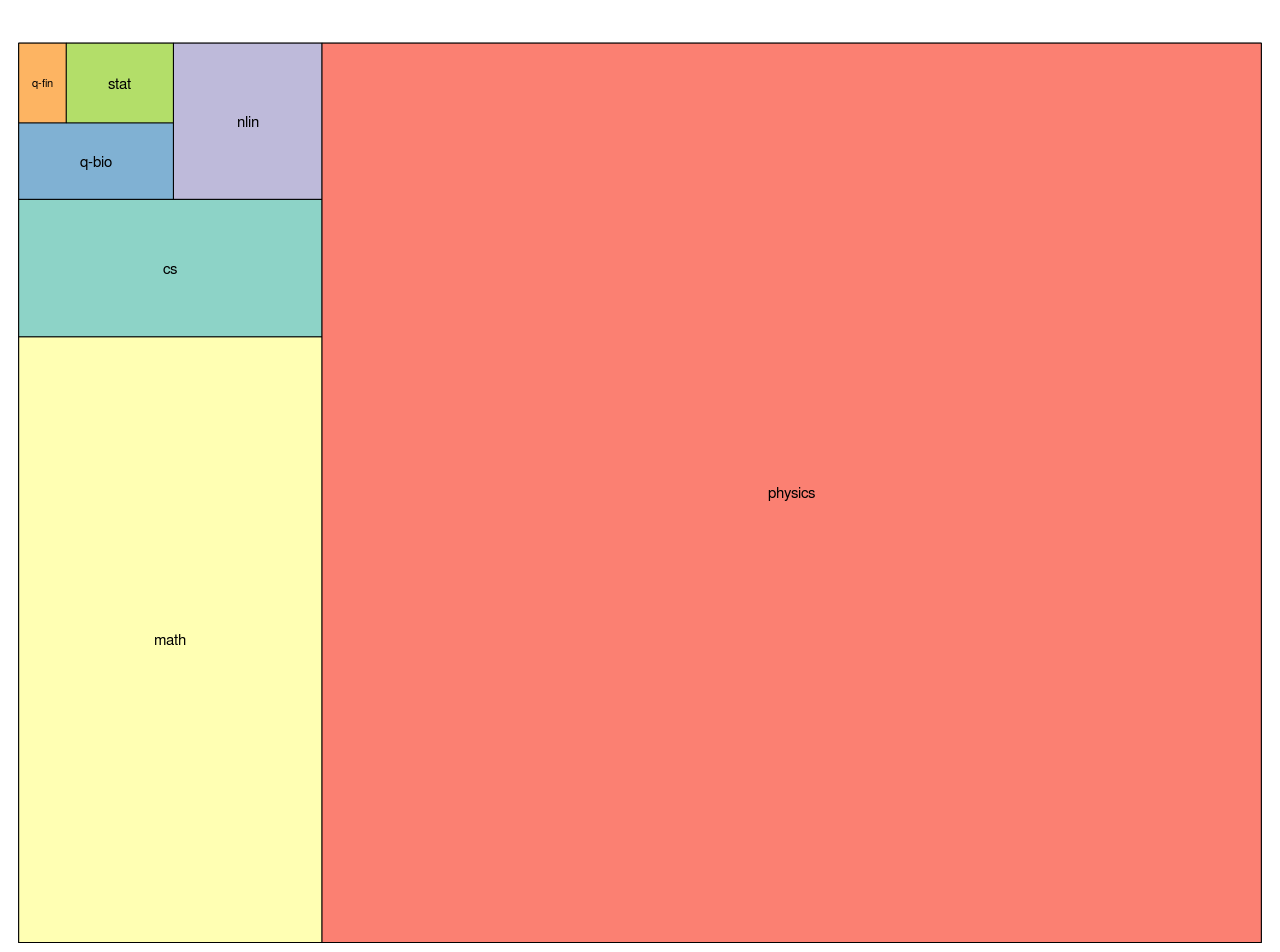
\includegraphics[scale=0.25]{../visual/treemap_no_title.png}
	\caption{Verteilung der Oberthemen}
	\label{treemap}
\end{figure}

\begin{table}[H]
\centering % used for centering table
\begin{tabular}{| l | l | l |}
	\hline
	Thema & Abk�rzung & Anteil(ca.) \\
	\hline
	Mathematics & math & $21.2 \%$ \\
	Condensed Matter & physics:cond-mat & $20.0 \%$\\
	Astrophysics & physics:astro-ph & $20.0\%$\\
	High Energy Physics - Phenomenology & physics:hep-ph & $13.0\%$\\
	High Energy Physics - Theory & physics:hep-th & $11.7\%$\\
	Physics & physics:physics & $6.8\%$\\
	Quantum Physics & physics:quant-ph &$6.3\%$\\
	General Relativity and Quantum Cosmology & physics:gr-qc & $6.0 \%$\\
	Computer Science & cs & $4.8 \%$ \\
	Mathematical Physics & physics:math-ph & $3.9 \%$\\
	Nuclear Experiment & physics:nucl-th & $3.8\%$\\
	High Energy Physics - Experiment & physics:hep-ex & $2.7\%$\\
	Nonlinear Sciences & nlin &  $2.7 \%$\\
	High Energy Physics - Lattice & physics:hep-lat & $2.1\%$\\
	Quantitative Biology & q-bio &$1.4 \%$ \\
	Nuclear Theory & physics:nucl-ex & $1.3\%$\\
	Statistics & stat & $1.0 \%$ \\
	Quantitative Finance & q-fin & $0.4\%$ \\
	Physics & physics & $0.0 \%$\\
	\hline
\end{tabular}
\caption{Aufteilung der Oberthemen im  Datensatz} % title of Table
\end{table}
Die durschnittliche Anzahl der vergebenen Themen betr�gt $1.3$ und die maximale Anzahl von Themen f�r eine Publikation ist $9$.
Bei rund $80 \%$ aller Publikationen wurde nur $1$ Thema im Kopfbereich eines Eintrages vergeben.
Bei $14 \%$ aller Themen wurden 2 und bei den restlichen $6 \%$ mehr als 2 Themen vergeben.


\subsection{Eigenschaften vom Thema Computer Science}
Zus�tzlich sollen alle Eintr�ge mit \textbf{cs} als Oberthema betrachtet werden und deren Themen im metadata-Teil untersucht werden.
Die Anzahl der wissenschaftlichen Publikationen mit dem Oberthema \textbf{cs} (Computer Science) betr�gt rund $34\;000$.
Die Bezeichnungen der Themen teilen sich in 2 gro�e Themengruppen auf.
Einerseits werden den Publikationen informatische und mathematische Klassen der Klassifikationsysteme ACM und MSC vergeben, was rund $30 \%$ der Informatikpublikationen betrifft, und andererseits wird eine hierarchische Unterteilung von arXiv.org verwendet, die aus $146$ Bezeichnern der Form ``Fachgebiet - Themengebiet'' z.B. ``Computer Science - Information Theroy'' besteht.
Die durschnittliche Anzahl von Themen pro Eintrag betr�gt hier $2.2$, was, unterm anderen, ein Indikator daf�r ist, dass es sinnvoll ist, Assoziationsregeln der Form $A \rightarrow B$ zu suchen.
\begin{figure}[H]
	\centering
	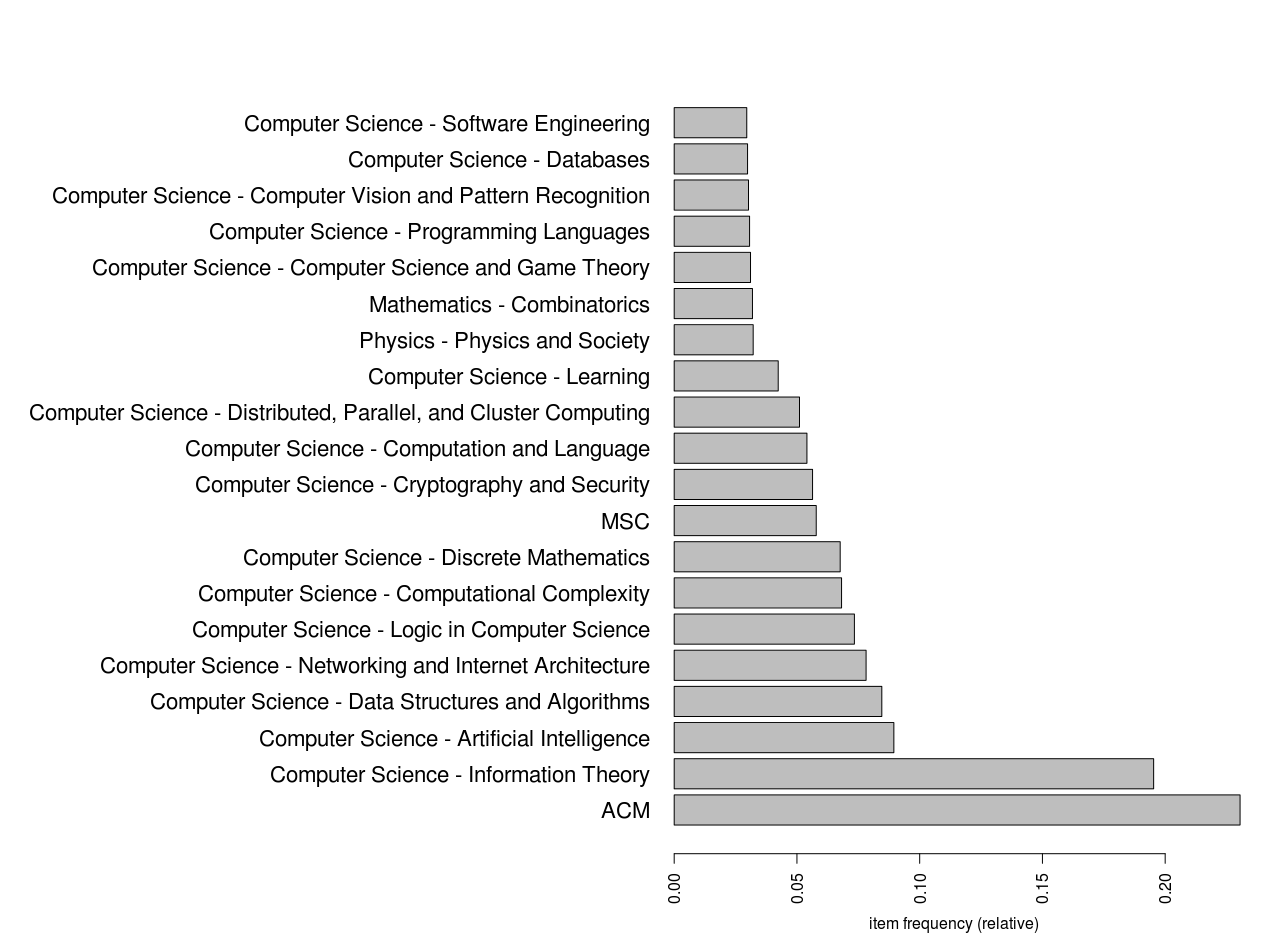
\includegraphics[scale=0.3]{../visual/horiCsFreq.png}
	\caption{Die 20 h�ufigsten Unterthemen bei Computer Science}
	\label{cs-freq}
\end{figure}

\section{Auswertung der Ergebnisse}
\subsection{Analyse der Oberthemen}
Zun�chst haben wir die Themen, die im Header jedes Eintrags einer Publikation auftreten, die sogenannten \PY{n+nt}{<setSpec}\PY{n+nt}{>}, untersucht.
Dabei konnten wir 19 einzigartige Themen feststellen, 13 davon waren Unterthemen der Physik.
Die anderen 6 waren wie folgt: $math$ (Mathematics), $cs$ (Computer Science), $nlin$ (Nonlinear Sciences), $q-bio$ (Quantitative Biology), $stat$ (Statistics) und $q-fin$ (Quantitative Finance).
Wir haben auf dem Gesamtdatensatz den apriori-Algorithums mit den Parametern $minsupp$ = 0.5\% und $minconf$ = 50\% angewandt, und dabei die folgenden 8 Assoziationsregeln(Tabelle \ref{tab:header}) gefunden. %cite table
Weiterhin haben wir die Unterthemen der Physik zusammengefasst und dann �berpr�ft, was f�r Assoziationsregeln sich ergeben.
Die Ergebnisse sind in Tabelle \ref{tab:headerCompact} dargestellt.

\subsubsection{Assoziationsregeln}
\begin{table}[H]
\centering % used for centering table
\begin{tabular}{| r l | l | l | l |}
		\hline
		\textbf{Regel}& &\textbf{Support} &\textbf{Konfidenz} & \textbf{Lift}\\
		\hline
		\{math\}  $\implies$ & \{stat\} & 0.6\% & 64\% &3.0  \\
		\{physics:math-ph\} $\implies$& \{math\} &3.8 \% & 100\% & 4.7 \\
		\{physics:hep-th, physics:math-ph\}  $\implies$& \{math\} &0.9 \% &100\% &4.7 \\
		\{math, physics:hep-th\}  $\implies$& \{physics:math-ph\}  &0.9 \% &63\% &16.3 \\
		\{physics:gr-qc, physics:hep-th\} $\implies$& \{physics:hep-th\} &0.6 \% &72 \% &6.1 \\
		\{physics:gr-qc, physics:hep-th\} $\implies$& \{physics:astro-ph\} &0.6 \% &70 \% &3.5 \\
		\{physics:gr-qc, physics:astro-ph\} $\implies$& \{physics:hep-th\} &0.9 \% &50 \%  &4.3 \\
		\{physics:astro-ph, physics:hep-th\} $\implies$& \{physics:gr-qc\}  &0.9 \% &74 \% &12.4 \\
		\hline
\end{tabular}
\caption{Assoziationsregeln der Oberthemen minsupp=0.5\% und minconf=50\%}
\label{tab:header}
\end{table}

\begin{table}[H]
\centering % used for centering table
\begin{tabular}{|rl|l|l|l|}
	\hline
	\textbf{Regel}& &\textbf{Support} &\textbf{Konfidenz} & \textbf{Lift}\\
	\hline
	$\{\emptyset\} \implies$ & \{physics\} & 78\% &78\% &1.0  \\
	\{stat\} $\implies$ & \{math\}  &0.6 \% &63 \% &3.0 \\
	\{nlin\} $\implies$ & \{physics\}  &1.3 \% &50 \% &0.64 \\
	\{math, nlin\} $\implies$ & \{physics\}  &0.4 \% &83 \% &1.1 \\
	\hline
\end{tabular}
 \caption{Assoziationsregeln mit zusammegefassten physics-Themen: Support 0.1 \% und Konfidenz 50 \%}
\label{tab:headerCompact}
\end{table}

\subsection{Analyse der Themen in den Metadaten}
\subsubsection{Assoziationsregeln}
Wie wir bereits gesehen haben, k�nnen wir anhand der Themen in den \PY{n+nt}{<setSpec}\PY{n+nt}{>} Attributen der Header relativ wenige interessante Informationen gewinnen.
Das liegt zu einem an der relativ geringen Anzahl von Themen, die pro Publikation vergeben wurden, und zum anderen daran, dass diese Themen viel zu allgemein sind.
Deshalb haben wir unsere weiteren Analysen auf die Subjects , die in den \PY{n+nt}{<dc: subject}\PY{n+nt}{>} Metadatentags auftauchen, aus dem Oberthema \textit{Computer Science} beschr�nkt.


Zun�chst haben wir den apriori-Algorithmus mit den Parametern $minsupp = 1\% $ und $ minconf = 50\%$ auf den \PY{n+nt}{<dc: subject}\PY{n+nt}{>} Tags aller Publikationen, deren Oberthema $Computer Science$ war, angewandt.
Dabei haben wir die folgenden 7 Regeln gewonnen (Tabelle \ref{tab:arules7}).
Bei einer n�heren Betrachtung dieser Regeln k�nnen wir Folgendes feststellen:\\
\begin{itemize}
\item Anhand von den $Support$-Werten k�nnen wir festhalten, dass es sich um Regeln handelt, die sich auf 400 bis 580 Datensatzeintr�ge beziehen.
\item Wir haben Themen nicht nur aus der Informatik, sondern auch solche, die zu der Physik oder der Mathematik geh�ren. Das liegt daran, dass die jeweiligen Publikationen auch Mathematik oder Physik in den \PY{n+nt}{<setSpec}\PY{n+nt}{>} Tags hatten. Diese Vermischung zeigt, dass es sich um Publikationen eines Randgebiets handelt - solche, die mehreren Forschungsrichtungen gleichzeitig zugeordnet werden k�nnen.
\item Zwei von den Regeln treten auch spiegelverkehrt auf: einmal in der Form $A \rightarrow B$, einmal in der Form $B \rightarrow A$. Dabei ist noch zu bemerken, dass sich die jeweiligen Paare nur um ihre Konfidenzwerte unterscheiden.
\item Es treten verschiedene Klassifikationen auf: sowohl diese von $arXiv.org$, als auch die $ACM$-Klassifikation. Solche ``vermischte'' Regeln k�nnen wir zur Herstellung von Mappings zwischen den Klassifikationen anwenden. Mehr dazu in \ref{sec:mappings}.
\end{itemize}

\begin{table}[H]
\centering % used for centering table
\begin{tabular}{|rl|l|l|l|}
	\hline
	\textbf{Regel}& &\textbf{sup} &\textbf{conf} &\textbf{lift}\\
	\hline
	\small I.2.7 $\implies$ &\small CS - Computation and Language &1.2\% &90 \% &16.9 \\
	\small CS- Systems and Control $\implies$ &  \small Math - Optimization and Control &1.5\% &88 \% &34 \\
	\small Math - Optimization and Control $\implies$ & \small CS - Systems and Control  &1.5\% &56 \% &34 \\
	\small CS - Social and Information Networks $\implies$ & \small Physics - Physics and Society &1.7\% &82 \% &25.5 \\
	\small Physics - Physics and Society $\implies$ & \small CS - Social and Information Networks &1.7\% &52 \% &25.5 \\
	\small F.4.1 $\implies$ & \small CS - Logic in Computer Science &1.6\% &78 \% &10.6 \\
	\small Math - Combinatorics $\implies$ & \small CS - Discrete Mathematics  &1.7\% &54 \% &7.9 \\
	\hline
\end{tabular}
 \caption{Assoziationsregeln der Unterthemen: Support 1 \% und Konfidenz 50 \%}
\label{tab:arules7}
\end{table}

F�r unsere weitere Analyse haben wir den $support$ Wert auf $0.1\%$ verringert.
Davon haben wir uns mehr Regeln erhofft, aufgrund deren mehrere Zusammenh�nge erkannt werden k�nnen.
Ein $support$ von $0.1\%$ bedeutet bei den knapp $34 000$ Publikationen mit dem Oberthema $Computer Science$ etwa $34$ Publikationen, f�r die eine gefundene Regel zutrifft.
Das haben wir als eine gute Basis eingesch�tzt, um spezifische Beziehungen zwischen einzelnen Themen aufzudecken.
Mit diesem Ansatz haben wir $218$ Assoziationsregeln gewonnen, die Top 10 von denen, jeweils nach einer der Assoziationsregelnkenngr��en sortiert, unten aufgef�hrt werden.
Unserer Einsch�tzung nach, decken diese Tabellen im gro�en und ganzen die interessantesten Regeln - diejenigen, die am h�ufigsten vorkommen (mit den h�chsten $supp$-Werten) und diejenigen, die am st�rksten sind (mit den h�chsten $conf$- und $lift$-Werten).
Weitere wichtige Regeln, die nicht zu den Top 10 geh�ren, aber trotzdem starke $Konfidenz$ und $Lift$ haben, werden in der Tabelle \ref{tab:otherRules} aufgef�hrt.

\begin{table}[H]
\centering % used for centering table
\begin{tabular}{|rl|l|l|l|}
	\hline
	\textbf{Regel}& &\textbf{sup} &\textbf{conf} &\textbf{lift}\\
	\hline
	\{D.2.9, J.1\} $\implies$ & \{H.4.1\} & $0.1\%$ &$ 100 \%$ & $473.0$\\
	\{D.2.9, H.4.1\} $\implies$ & \{J.1\} & $0.1\%$ & $100 \%$ & $500.8$\\
	\{D.2.9, J.1\} $\implies$ & \{K.6.4\} & $0.1\%$ & $100 \%$ & $479.6$\\
	\{J.1, K.6.4\} $\implies$ & \{D.2.9\} & $0.1\%$ & $100 \%$ & $577.2$\\
	\{D.2.9, H.4.1\} $\implies$ & \{K.6.4\} &$0.1\%$ & $100 \%$ & $479.6$\\
	\{J.1, K.6.4\} $\implies$ & \{H.4.1\} & $0.1\%$ & $100 \%$ & $473.0$\\
	\{H.4.1, K.8.1\} $\implies$ & \{K.6.4\} &$ 0.2\%$ & $100 \%$ & $479.6$\\
	\{K.6.4, K.8.1\} $\implies$ & \{H.4.1\} &$ 0.2\%$ & $100 \%$ & $473.0$\\
	\{D.2.5,K.8.1\} $\implies$ & \{H.4.1\}  &$ 0.1\%$ & $100 \%$ & $473.0$\\
	\{D.2.5, H.4.1\} $\implies$ & \{K.8.1\} &$0.1\%$ & $100 \%$ & $567.6$\\
	\hline
\end{tabular}
 \caption{Assoziationsregeln der Unterthemen sortiert nach Konfidenz mit:  Support 0.1 \% und Konfidenz 50 \%}
\end{table}

\begin{table}[H]
\centering % used for centering table
\begin{tabular}{|rl|l|l|l|}
	\hline
	\textbf{Regel}& &\textbf{sup} &\textbf{conf} &\textbf{lift}\\
	\hline
	\{J.1, K.6.4\} $\implies$ &\{D.2.9\} &0.1\% & 100 \% & 577.2 \\
	\{H.4.1, J.1, K.6.4\} $\implies$ & \{D.2.9\} &0.1\%& 100\% & 577.2\\
	\{D.2.5, H.4.1\} $\implies$ & \{K.8.1\} &0.1\%& 100\% & 567.6\\
	\{D.2.5, K.6.4\} $\implies$ & \{K.8.1\} &0.1\%& 100\% & 567.6\\
	\{D.2.5, H.4.1, K.6.4\} $\implies$ & \{K.8.1\} &0.1\%& 100 \% & 567.6\\
	\{H.4.1, J.1\} $\implies$ & \{D.2.9\} &0.1\%& 92.7 \% & 534.9\\
	\{D.2.9, H.4.1\} $\implies$ & \{J.1\} &0.1\%& 100 \% & 500.8\\
	\{D.2.9, H.4.1, K.6.4\} $\implies$ & \{J.1\} &0.1\%& 100\% & 500.8\\
	\{D.2.9, K.6.4\} $\implies$ & \{J.1\} &0.1\%& 97.4\% & 487.9\\
	\{D.2.9, J.1\} $\implies$ & \{K.6.4\} &0.1\%& 100\% & 479.6\\
	\hline
\end{tabular}
 \caption{Assoziationsregeln der Unterthemen sortiert nach Lift mit:  Support 0.1 \% und Konfidenz 50 \%}
\end{table}

\begin{table}[H]
\centering
\begin{tabular}{|rl|l|l|l|}
	\hline
	\textbf{Regel} & &\textbf{sup} &\textbf{conf} &\textbf{lift}\\
	\hline
	\small Math - Combinatorics $\implies$ & \small CS - Discrete Mathematics  &1.7\% &54 \% &7.9 \\
	\small CS - Social and Information Networks $\implies$ & \small Physics - Physics and Society &1.7\% &82 \% &25.5 \\
	\small Physics - Physics and Society $\implies$ & \small CS - Social and Information Networks &1.7\% &52 \% &25.5 \\
	\small F.4.1 $\implies$ & \small CS - Logic in Computer Science &1.6\% &78 \% &10.6 \\
	\small CS- Systems and Control $\implies$ & \small Math - Optimization and Control &1.5\% &88 \% &34 \\
	\small I.2.7 $\implies$ & \small CS - Computation and Language &1.2\% &90 \% &16.9 \\
	\small Math - Optimization and Control $\implies$ & \small CS - Systems and Control  &1.5\% &56 \% &34 \\
	\small I.2.7(Natural Language Processing)  $\implies$ & \small CS - Computation and Language  &1.2\% &91 \% &16.9 \\
	\small G.2.2(Graph Theory)   $\implies$ & \small CS - Discrete Mathematics  &0.8\% &59 \% &8.8 \\
	\small F.1.3(Complexity Measures)  $\implies$ & \small CS - Computational Complexity  &0.7\% &86 \% &12.6 \\
	\hline
\end{tabular}
 \caption{Assoziationsregeln der Unterthemen sortiert nach Support mit:  Support 0.1 \% und Konfidenz 50 \%}
\end{table}

\begin{table}[H]
\centering % used for centering table
\begin{tabular}{|rl|l|l|l|}
	\hline
	\textbf{Regel}& &\textbf{sup} &\textbf{conf} &\textbf{lift}\\
	\hline
	\{D.2.5, K.6.4\} $\implies$ &\{H.4.1\} &0.1\% & 100 \% & 473.0 \\
	\{D.2.9, J.1, K.6.4\} $\implies$ & \{H.4.1\} &0.1\%& 100\% & 473.0\\
	\{D.2.5, K.6.4, K.8.1\} $\implies$ & \{H.4.1\} &0.1\%& 100\% & 473.0\\
	\{D.2.9, K.6.4\} $\implies$ & \{H.4.1\} &0.1\%& 97.4\% & 460.8\\
	\{K.6.4\} $\implies$ & \{H.4.1\} &0.2\%& 93 \% & 439.7\\
	\{H.4.1, J.1\} $\implies$ & \{K.6.4\} &0.1\%& 92.7 \% & 444.5\\
	\{K.8.1\} $\implies$ & \{H.4.1\} &0.2\%& 91.7 \% & 433.5\\
	\{K.8.1\} $\implies$ & \{K.6.4\} &0.2\%& 91.7\% & 439.7\\
	\{H.4.1\} $\implies$ & \{K.6.4\} &0.2\%& 91.7\% & 439.7\\
	\{H.4.1, K.6.4\} $\implies$ & \{K.8.1\} &0.2\%& 83.3\% & 473.0\\
	\hline
\end{tabular}
 \caption{Weitere Assoziationsregeln der Unterthemen mit hohen Lift- und Konfidenzwerten}
\label{tab:otherRules}
\end{table}


\subsubsection{Mappings zwischen Klassifikationen}
\label{sec:mappings}
Die in der folgenden Tabelle dargestellten Regeln sind alle Assoziationsregeln, wo genau ein ACM-Thema auf der linken Seite und ein arxiv-Thema auf der rechten Seite steht.
Wir haben explizit nach Regeln, die diese Form haben, gesucht, damit eine eindeutige Abbildung zwischen Subjects in der jeweiligen Klassifikationen m�glich ist.
Wir haben keine Regeln der Form $arxiv \rightarrow ACM$ gefunden, was auch logisch ist, da die ACM-Klassifikation eine viel feinere Unterteilung als arxiv anbietet.
Alle gefundenen Regeln haben relativ hohe Konfidenz- und Liftwerte, was daf�r spricht, dass die so entstandenen Mappings zuverl�ssig sind.

\begin{table}[H]
\centering % used for centering table
\begin{tabular}{|rl|c|c|c|}
	\hline
	\textbf{Regel(ACM $\implies$ }  &\textbf{arXiv.org)} & {Support} &\textbf{Konfidenz} & \textbf{Lift}\\
	\hline
	\small G.4(Mathematical Software) $\implies$ & \small CS - Mathematical Software & 0.1\% &51\% &67.4  \\
	\small K.4.m(Computers and Society) $\implies$ & \small CS - Computers and Society &0.2 \% &96 \%  &53.4 \\
	\small I.2.9(Robotics) $\implies$ & \small CS - Robotics &0.1 \% & 75 \%  &52.1 \\
	\small H.3.7(Digital Libraries) $\implies$ & \small CS - Digital Libraries &0.3 \% &89 \% &48.7 \\
	\small I.1.2(Symbolic Manipulation - Algorithm) $\implies$ & \small CS - Symbolic Computation  &0.1 \% &60 \%  &41.3 \\
	\small I.2.11(Distributed Artificial Intelligence) $\implies$ & \small CS - Multiagent Systems  &0.2 \% &53 \%  &35.9 \\
	\small H.5.2(User Interfaces) $\implies$ & \small CS - Human-Computer Interaction &0.2 \% &58 \%  &33.7 \\
	\small I.3.5(Computational Geometry) $\implies$ & \small CS - Computational Geometry &0.3 \% &88 \%  &31.2 \\
	\small H.2.3(Datebase Managment - Languages) $\implies$ & \small CS - Databases &0.2 \% &91 \%  &30.6 \\
	\hline
\end{tabular}
 \caption{Assoziationsregeln der Unterthemen: Support 0.1 \% und Konfidenz 50 \%}
\end{table}
\subsubsection{zeitliche Analyse gefundener Regeln}
Die zeitliche Betrachtung der Regeln macht es m�glich die Entwicklung der Themen und die Korrelation von Themen f�r wissenschaftliche Publikationen zu beobachten. Mehrere Szenarien sind f�r die Entwicklung denkbar:
\begin{enumerate}
	\item Themengebiete k�nnen verschmelzen
	\item ein Thema kann sich in verschiedene Gebiete aufteilen
	\item Themen k�nnen verschwinden oder entstehen
\end{enumerate}

Im folgenden werden die Szenarien Verschmelzung und Entstehung betrachtet, die bei der Analyse der zeitliche Entwicklung der Regeln aus Tabelle \ref{tab:arules7} entstanden sind.

Als erstes wird der zeitliche Verlauf der Regel \textbf{Computer Science - Systems and Control} $\implies$ \textbf{Mathematics - Optimization and Control} betrachtet.
\begin{figure}[H]
	\centering
	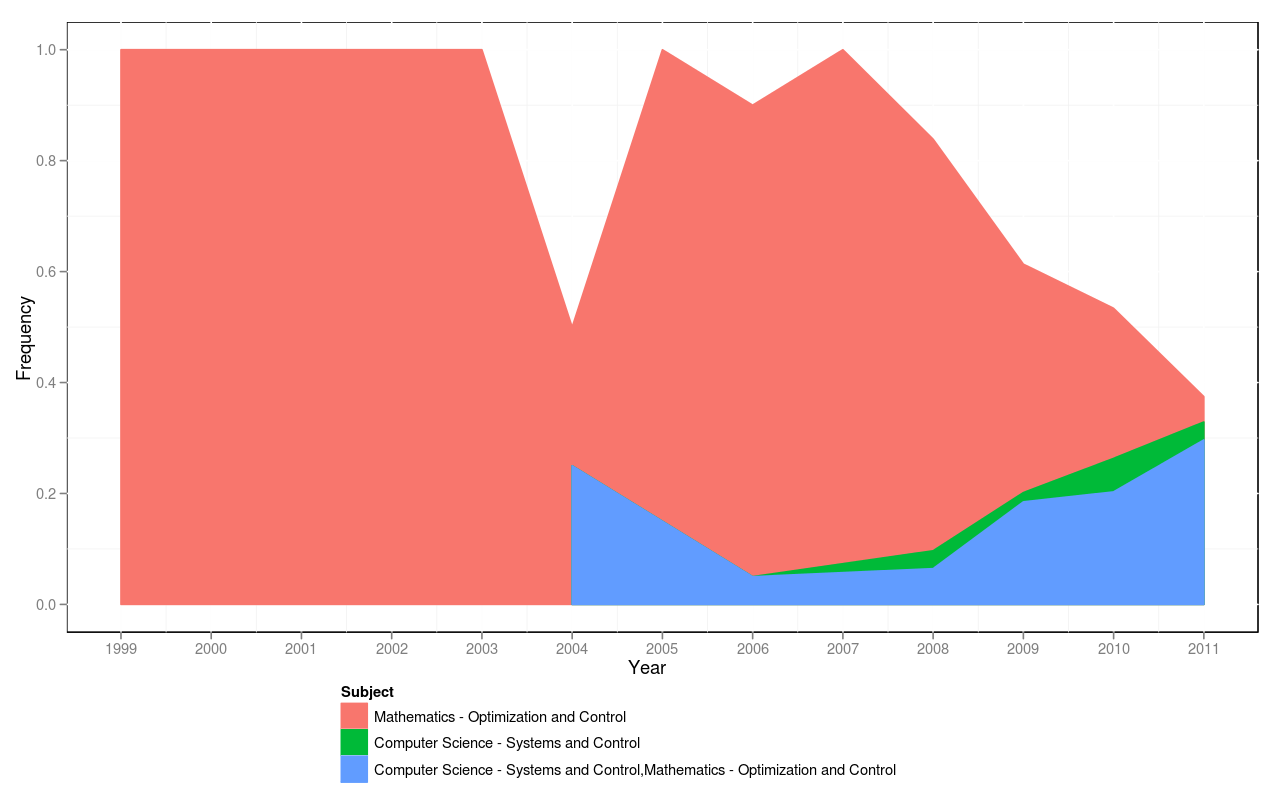
\includegraphics[scale=0.425]{../visual/trend/csmathscaled.png}
	\caption{Entstehung eines Themas}
	\label{fig:csmath}
\end{figure}
In Abbildung \ref{fig:csmath} ist zu erkennen, dass vor dem Jahr 2004 nur Publikationen mit dem Thema Optimization and Control der Mathematik ver�ffentlicht wurden, aber keine mit dem Thema System and Control in der Informatik.
Vom Jahr 2004 bis 2006 ist zu sehen, dass nun alle Publikationen im Themengebiet Computer Science - System and Control immer im Zusammenhang mit dem Thema Mathematics - Optimization and Control ver�ffentlicht wurden. Ab dem Jahr 2006 erh�ht sich die Anzahl der ver�ffentlichen Publikationen mit dem Thema Computer Science - System and Control kontinuierlich auch ohne dem Thema aus der Mathematik, das sich im gleichen Zeitraum deutlich seltener vergebenen wurde, als in den Jahren davor. Anhand des zeitlichen Verlauf l�sst sich also feststellen, das sich das Interesse teilweise vom Thema Opimization and Control zum Thema System and Control verschoben hat und das Thema System and Control der Informatik in irgendeiner Form aus dem Thema Optimization and Control der Mathematik entwickelt hat.

Als n�chstes Betrachten wir die zeitliche Entwicklung der Regel \textbf{Computer Science - Social and Information Networks} $\implies$ \textbf{Physics - Physics and Society}.
\begin{figure}[H]
	\centering
	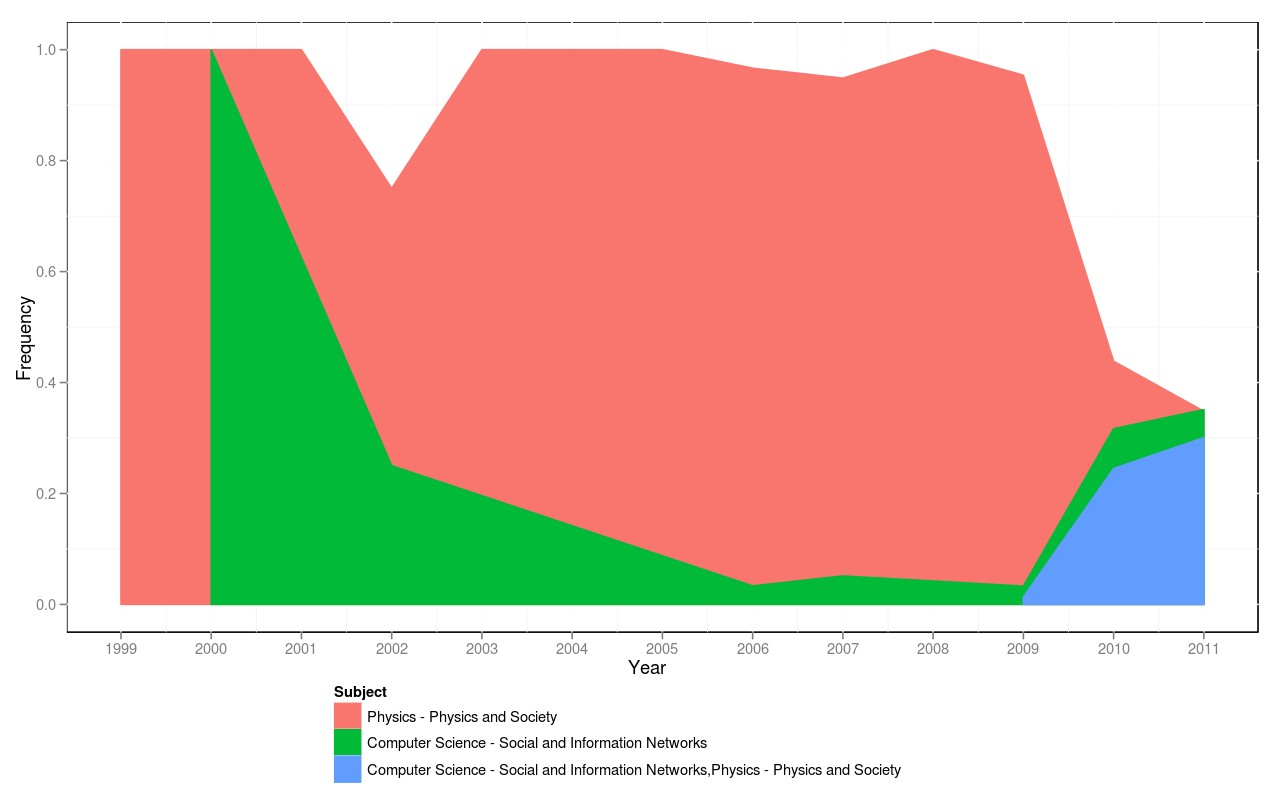
\includegraphics[scale=0.425]{../visual/trend/csphscaled.png}
	\caption{Verschmelzung von Themen}
	\label{csph}
\end{figure}
Bis zum Jahr 2009 werden die beiden Themen unabh�ngig vergeben und es zeigt sich keine Korrelation der beiden Themengebiete. Erst ab dem Jahr 2009 werden beide Themen bei Publikationen zusammen vergeben. Dazu kommt eine schneller Anstieg bei der gemeinsamen Vergabe und der ebenso deutliche Abfall bei der H�ufigkeit des Themas Physics - Physics and Society. Dies l�sst einen starken Zusammenhang zwischen beiden Themen vermuten. Und da das Thema Computer Science - Social and Information Networks im gleichem Zeitraum einen deutlichen Anstieg zeigt, kann von einer gro�en �berschneidung der Themengebiete ausgegangen werden. Auch historisch l�sst sich die Entwicklung einordnen. Mit dem entstehen von sozialen Netzwerken im Internet hat auch die Erforschung ebendieser in der Informatik an Interesse gewonnen. Die besteht also die M�glichkeit, dass sich die Informatik die Verfahren der Physik in diesem Themengebiet bedient hat und das in der Physik ebenfalls Interesse an diesen Netzwerken entstanden ist, sodass sich beide Themengebiete st�rker austauschen udn zusammenarbeiten.

\section{Further Research und m�gliche Anwendung}

%further research:
%normalisierte zeitliche analyse; vergleich zum ganzen
%kombination von themen und key words im titel/abstract bei der Assoziationsanalyse
%
%anwendungen:
%mappings
%tag / subject vorschlag systeme
%recommender systeme f�r papers

\subsection{Weiterf�hrende Untersuchungen}
Wir haben im Rahmen unseres Projekts viele bedeutende Zusammenh�nge aufgedeckt.
Allerdings gibt es noch ein paar interessante Aspekte, denen wir, vor allem aufgrund zeitlichen Mangel, nicht nachgegangen sind.

F�rs Erste w�re es spannend, die zeitliche Entwicklung mehreren im Datensatz vorkommenden Themen und der darauf basierenden Regeln zu untersuchen.
Wie wir anhand von 2 Beispielen gesehen haben, kann diese Analyse lukrative Ergebnisse �ber die Entwicklung der Themen, deren Entstehung, Verschwinden, Spaltung oder Verschmelzung, im Allgemeinen deren Aktualit�t liefern.

Eine weitere n�tzliche Untersuchung w�re, andere Faktoren in unsere Analyse mit einzubeziehen.
Man k�nnte studieren, welche Assoziationsregeln sich ergeben, wenn nicht nur die vergebenen Themen, sondern auch Schl�sselw�rter aus dem Titel oder Abstract oder die Autoren der Publikation betrachtet werden.
So k�nnen zus�tzliche Erkenntnisse gewonnen werden, z.B. welche Autoren in welchen Themengebieten besonders wichtig sind, oder welche Begriffe mit einem Thema assoziiert werden.

\subsection{Anwendungen}
Die in unserer Analyse gefundenen Assoziationsregeln k�nnen auf mehreren Weisen verwendet werden.
Eine m�gliche Anwendung - die Erstellung von Mappings zwischen verschiedenen standardisierten Klassifikationen, wurde bereits im Kapitel 4 angedeutet.
Diese k�nnen beim Hochladen von Publikationen in verschiedene wissenschaftliche Datenbanken sehr n�tzlich sein.
Wenn sinnvolle und zuverl�ssliche Abbildungen zwischen verschiedenen Klassifikationen ermittelt werden, k�nnten die f�r ein Paper in einer Notation vergebene Themen automatisch in eine andere �berf�hrt werden.
Ferner k�nnen solche Mappings und Assoziationsregeln generell f�r das Entwickeln eines Vorschlagsystems f�r Themen verwendet werden.
Ein solches System wird in der Lage sein, einem Nutzer, der seine Arbeit online stellt und mit Themen kennzeichnet, geeignete Vorschl�ge f�r weitere Themen, die relevant sein k�nnten, oder ihre entsprechenden Formulierungen in einer anderen Klassifikation zu machen.
Eine weitere Anwendung von Assoziationsregeln kann im Entwurf von Paperrecommendersystemen gefunden werden.
Zweck dieser Systeme ist es, einer Leserin, die ein Paper interessant gefunden hat, weitere relevante/verwandte Arbeiten anzubieten.
F�r das Gestalten so eines Systems werden auch genau solche Assoziationsregeln relevant, die nicht so oft auftreten (einen niedrigen $\mathrm{support}$ haben), daf�r aber relativ stark sind (h�here $\mathrm{confidence}$ und $\mathrm{lift}$ Werte haben).
Dann werden der Nutzerin eine geringe Anzahl an Publikationen mit hoher Relevanz angeboten.

\section{Zusammenfassung}
Wie in dieser Ausarbeitung gezeigt, ist die Assoziationsanalyse der Themen wissenschaftlicher Publikationen eine wichtige Methode der bibliometrischen Untersuchungen.
Durch die Betrachtung der vergebenen Subjects f�r den arxiv-Datensatz haben wir bedeutende Erkenntnisse �ber die Verwandschaft manchen Themen als auch �ber die Entwicklung �ber die Zeit von bestimmten Themengebieten gewonnen.
Anlehnend an die Ergebnisse, die dieses Paper pr�sentiert, k�nnen standardisierten Mappings zwischen verschiedenen Klassifikationen, Themenvorschlag- sowie Paperrecommendersysteme entwickelt werden.
Um diese erfolgreich umzusetzen, bietet sich an, neben der Assoziationsanalyse von Themen auch weitere Methoden, wie z.B. Autorenanalyse oder Untersuchung der Schl�sselw�rter des Titels und/oder des Abstracts, zu verwenden.

%* was gewinnen wir durch Assoziationsanalyse von Themen
%* was haben wir gemacht
%* hinweis auf weiterf�hrende recherche

%In a general way,
%
%restate your topic and why it is important,
%restate your thesis/claim,
%address opposing viewpoints and explain why readers should align with your position,
%call for action or overview future research possibilities.
%
%from my specific topic to more general matters
%say what you have already said but do it quickly, sharply and in different words


\nocite{*}
%\nocite{HasChe11}
%\nocite{DBLP:journals/jmlr/HahslerCHB11}
%\nocite{HahGruHorBuc11}
\newpage

\bibliographystyle{lni}
\bibliography{lnitemplate}

\end{document}
